\section{Setting and partition bound}
\label{sec:setting}
Let $\d\ge2$ and let $\muunif$ be normalized Lebesgue measure on $\T^\d=\R^\d/\Z^\d$.  The mean-zero periodic logarithmic kernel is normalized by
\begin{equation}
 \wh\g(k)=\frac{c_\d}{(2\pi|k|)^\d}\quad(k\ne0),
 \qquad c_\d=2^{\d-1}\pi^{\d/2}\Gamma(\d/2),
 \qquad \g(x)=-\log|x|+O_\d(1)
 \quad(x\to0).
 \label{eq:kernel-normalization}
\end{equation}
Here, $\wh f(k)=\int f(x)e^{-2\pi ik\cdot x}\,\dd\muunif(x)$ and $\wh\g(0)=0$.
For independent $X_1,\ldots,X_N$ with law $\muunif$, set
\begin{equation}
 \mathsf W_N(K)\coloneqq\frac1N\sum_{i\ne j}K(X_i,X_j),
 \qquad
 Z_{N,\be}\coloneqq\E\big[e^{\frac\be2\mathsf W_N(\g)}\big],
 \label{eq:homogeneous-partition-function}
\end{equation}
where a function of one variable denotes the translation-invariant kernel $K(x-y)$.

Our only macroscopic assumption is the log-HLS inequality: for some $B\in(0,2\d]$,
\begin{equation}
 \Hr(\rho\muunif\mid\muunif)
 \coloneqq\int\rho\log\rho\,\dd\muunif
 \ge\frac B2\iint\g(x-y)(\rho(x)-1)(\rho(y)-1)
                  \,\dd\muunif(x)\dd\muunif(y)
 \label{eq:strict-subcritical-macroscopic-inequality}
\end{equation}
for every probability density of finite entropy.  No value or optimality of $B$ is needed.

\begin{thm}[Uniform partition bound]
\label{thm:principal}
Under \eqref{eq:strict-subcritical-macroscopic-inequality}, for every $0\le\be_0<B$ there is a finite constant $C=C(\d,B,\be_0)$ such that
\begin{equation}
 \sup_{N\ge2}\sup_{0\le\be\le\be_0}Z_{N,\be}\le C.
 \label{eq:principal-order-one}
\end{equation}
\end{thm}

The proof has three ingredients.  A positive-definite cutoff (Section~\ref{sec:physical-cutoff-proof}) splits $\g$ into a smooth bulk $b_r$ and a singular part $\widetilde s_r$ supported within distance $r$ of the diagonal, both positive semidefinite.  The bulk inherits \eqref{eq:strict-subcritical-macroscopic-inequality} and is controlled by a continuous-kernel entropy bound (Lemma~\ref{lem:continuous-entropy-partition}).  The singular part is perturbative as long as no box of side $2r$ is overcrowded: a particle then interacts through $\widetilde s_r$ with only a small fraction of the others, and a moment estimate for centered arrays of independent variables (Lemma~\ref{lem:canonical-array-exponential}) applies.  The overcrowded event has exponentially small probability and can compensates a trivial exponentially growing bound for the partition function (Section~\ref{subsec:proof-bad-set}).

\textbf{Boxes and the good event.}
For an integer $J\ge3$, partition the torus into
\begin{equation}
 A_a=J^{-1}(a+[0,1)^\d),\qquad
 a\in(\Z/J\Z)^\d,\qquad M=J^\d.
 \label{eq:common-box-partition}
\end{equation}
Write $L_i=a$ when $X_i\in A_a$, and $n_a=\#\{i:L_i=a\}$.
Let $\nu_a=M\one_{A_a}\muunif$ be the uniform probability measure on $A_a$, and let $Q_J$ denote box averaging: $(Q_Ju)|_{A_a}=\int u\,\dd\nu_a$.
Both parts of the proof use this grid, at a resolution independent of $N$: the singular part at the resolution tied to the cutoff below, and the bulk part (Appendix~\ref{app:continuous-proof}) at a finer resolution chosen after $r$ has been fixed.

For the singular part, fix $0<\delta<1$ and choose the cutoff and the occupancy event together:
\begin{equation}
 r=\frac1{2J},\qquad
 \mathcal A_{N,J,\delta}=\{n_a\le\delta N\ \text{for every }a\},
 \qquad
 \mathcal B_{N,J,\delta}=\mathcal A_{N,J,\delta}^{\mathsf c}.
 \label{eq:physical-neighbor-events}
\end{equation}
The singular kernel constructed in Section~\ref{sec:physical-cutoff-proof} is supported at distance at most $r$.
Nonadjacent boxes are separated by at least $J^{-1}=2r$, so only particles in the same box or in adjacent boxes interact through it.  Here, adjacency includes shared faces, edges, and corners, with periodic labels, so each box has $3^\d-1$ neighbors.
On $\mathcal A_{N,J,\delta}$, one box contains at most $\delta N$ particles and two boxes at most $2\delta N$; see Figure~\ref{fig:periodic-cell-pair-band}.

\begin{figure}[htbp]
\centering
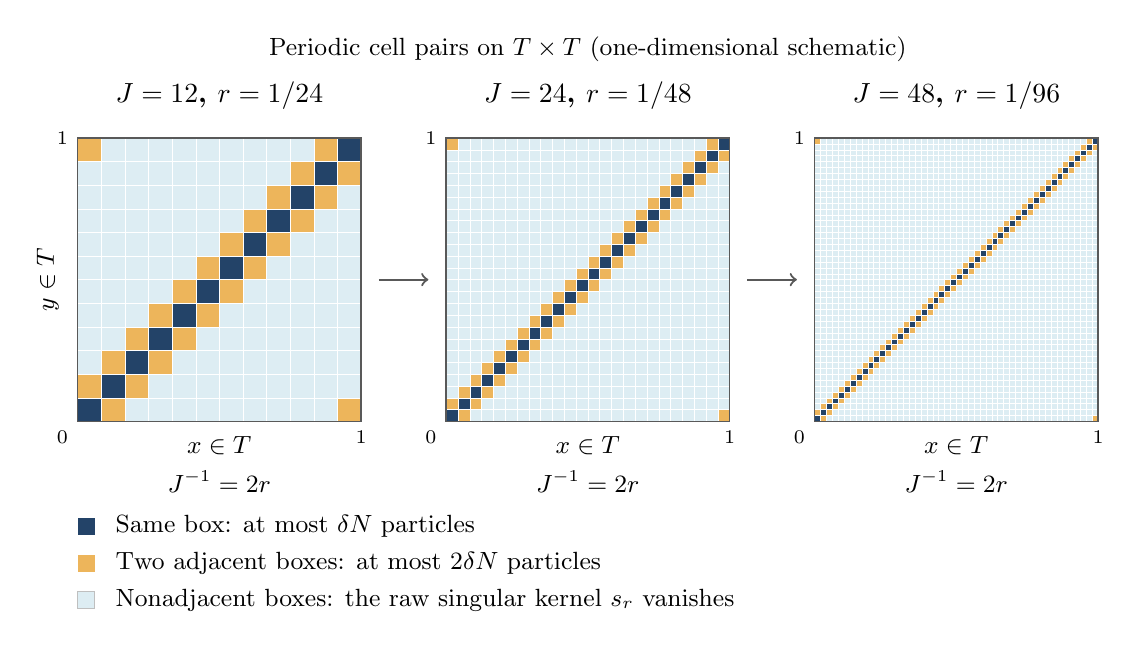
\begin{tikzpicture}[x=.9cm,y=.9cm,font=\small]
\node at (7.2,5.25) {Periodic cell pairs on $\mathbb T\times\mathbb T$ (one-dimensional schematic)};
\definecolor{cellself}{RGB}{35,67,104}
\definecolor{cellnear}{RGB}{237,181,91}
\definecolor{cellfar}{RGB}{221,237,243}
\foreach \cells/\shift/\cutoff in {12/0/{1/24},24/5.2/{1/48},48/10.4/{1/96}} {
 \begin{scope}[shift={(\shift,0)}]
  \node[font=\bfseries] at (2,4.6) {$J=\cells$, $r=\cutoff$};
  \fill[cellfar] (0,0) rectangle (4,4);
  \pgfmathtruncatemacro{\lastcell}{\cells-1}
  \foreach \a in {0,...,\lastcell} {
   \foreach \offset in {-1,1} {
    \pgfmathtruncatemacro{\b}{mod(\a+\offset+\cells,\cells)}
    \fill[cellnear] ({4*\a/\cells},{4*\b/\cells}) rectangle ({4*(\a+1)/\cells},{4*(\b+1)/\cells});
   }
   \fill[cellself] ({4*\a/\cells},{4*\a/\cells}) rectangle ({4*(\a+1)/\cells},{4*(\a+1)/\cells});
  }
  \foreach \a in {0,...,\cells} {
   \draw[white,line width=.13pt] ({4*\a/\cells},0)--({4*\a/\cells},4);
   \draw[white,line width=.13pt] (0,{4*\a/\cells})--(4,{4*\a/\cells});
  }
  \draw[black!65,line width=.5pt] (0,0) rectangle (4,4);
  \node[below left,font=\scriptsize] at (0,0) {$0$};
  \node[below,font=\scriptsize] at (4,0) {$1$};
  \node[left,font=\scriptsize] at (0,4) {$1$};
  \node[below] at (2,-.08) {$x\in\mathbb T$};
  \ifnum\cells=12\node[rotate=90] at (-.42,2) {$y\in\mathbb T$};\fi
  \node at (2,-.85) {$J^{-1}=2r$};
 \end{scope}
}
\foreach \shift in {0,5.2} {\draw[->,thick,black!65] ({4.25+\shift},2)--({4.95+\shift},2);}
\fill[cellself] (0,-1.6) rectangle (.24,-1.36);
\node[anchor=west] at (.4,-1.48) {Same box: at most $\delta N$ particles};
\fill[cellnear] (0,-2.12) rectangle (.24,-1.88);
\node[anchor=west] at (.4,-2) {Two adjacent boxes: at most $2\delta N$ particles};
\fill[cellfar,draw=black!25] (0,-2.64) rectangle (.24,-2.4);
\node[anchor=west] at (.4,-2.52) {Nonadjacent boxes: the raw singular kernel $s_r$ vanishes};
\end{tikzpicture}

\caption{The grid is chosen to match the singular cutoff: the cell side is $2r$.  In this one-dimensional schematic, $s_r(x-y)$ can be nonzero only in a diagonal square or in one of its two neighboring squares, including the periodic corner squares.  The colored boxes cover its support; they are not all filled by it.  Refining the grid and reducing $r$ together narrows the band while keeping three possible partner boxes per box, the box itself included ($3^\d$ in dimension $\d$).}
\label{fig:periodic-cell-pair-band}
\end{figure}
